\chapter{Trial Results} 
\label{chap:trialResults}
%in this section i will first discuss the raw results of the trial, then discuss both the primary results (the raw data) and the secondary results (lessons on how the trial was run)

\section {Limitations of Trial}
The scope of the exploratory trial was limited after the Dissertation proposal due to timing of applicable grants. Some parts of the proposed design, including detection of PIPs, generation of targeted interventions, and wireless data delivery were reduced as a result, in scale in order to comply with the timing demands enforced by the supporting grants. The project was refocused on collecting physiologic and psychosocial data and post processing that data. The BKE was scrapped as a live updating entity, eliminating the requirement for a medical ontology.

The goal of the trial, was now to build and implement a system for data collection consisting of a non-intrusive sensor apparatus to collect psychometric data and a cellphone application to accumulate psychosocial data. The sensor would need to have its data manually downloaded each week by a visiting clinician. Detailed information about the sensor package can be found in \cref{chap:ProtoTypeBuildTest} : \nameref{chap:ProtoTypeBuildTest} .


\section{Exploratory Trial Initial Description}

Sethares et al. proposed a trial to assess the usefulness of the sensor design concepts including both the new sensor hardware and the cellphone application to collect somatic awareness data.  The trial was originally proposed to run from November 2013 through August 2014 \cite{KristenASethares2013}. Due to issues unrelated to research the first patient was not equipped with sensors until May 2014.

\begin{figure}
 \begin{center}
  \label{fig:CarePackage}
  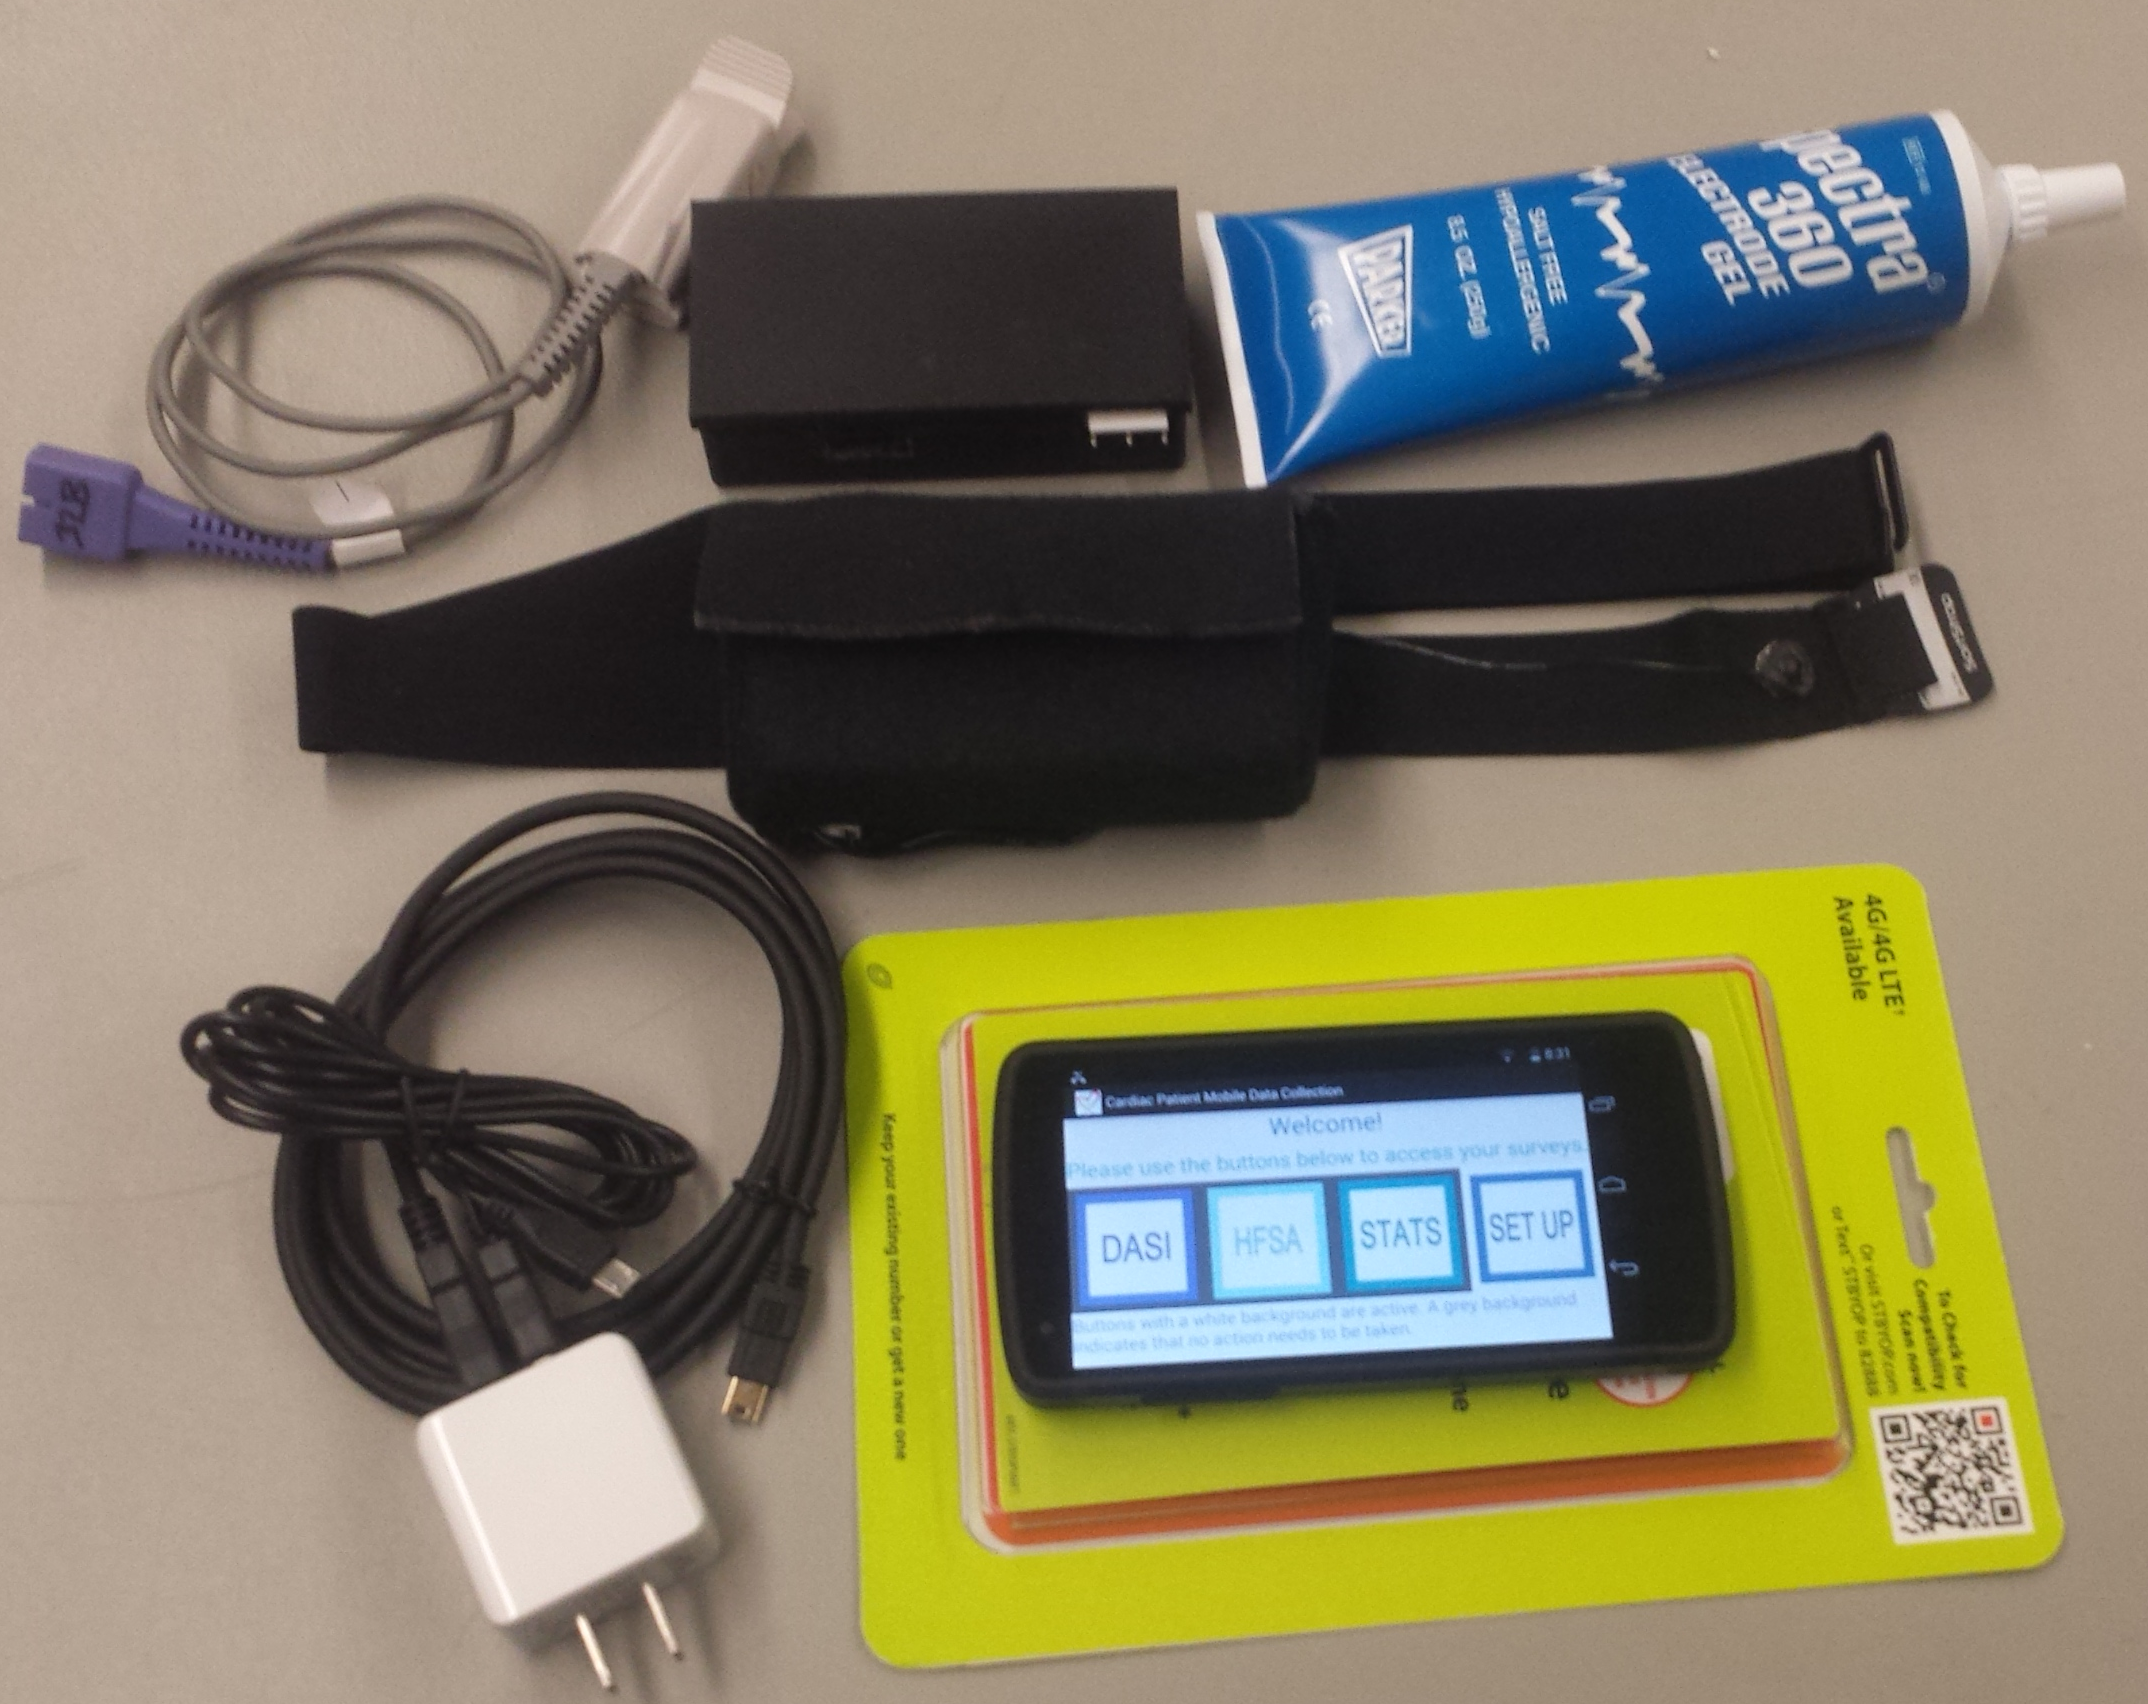
\includegraphics[scale=1,width=0.75\textwidth]{Images/carePackage.png} 
  \caption{Care Package for each Participant.} 
 \end{center}
\end{figure}



Each participant was provided with a package as shown in \cref{fig:CarePackage}:
\begin{itemize}
\item An lg nexus 5 cellphone with the heart monitor application
\item a sensor assembly
	\begin{itemize}
	\item a 3d printed enclosure
	\item a sensor board
	\item a modified polar(r) brand chest strap
	\item a fabric pouch
	\end{itemize}
\item a tube of electrode gel
\item a two port USB charger
\item a USB A to USB mini cable
\item a USB A to USB micro cable
\end{itemize}

The patient was instructed to wear the device during the day and to wear the finger clip, when convenient. The patient was instructed to take off the device and plug it in to charge at night . Additionally, the patient was given a smartphone, with a data plan, and shown how to use the survey application (app). 

\begin{figure}
 \begin{center}
  \label{fig:AndroidSplash}
  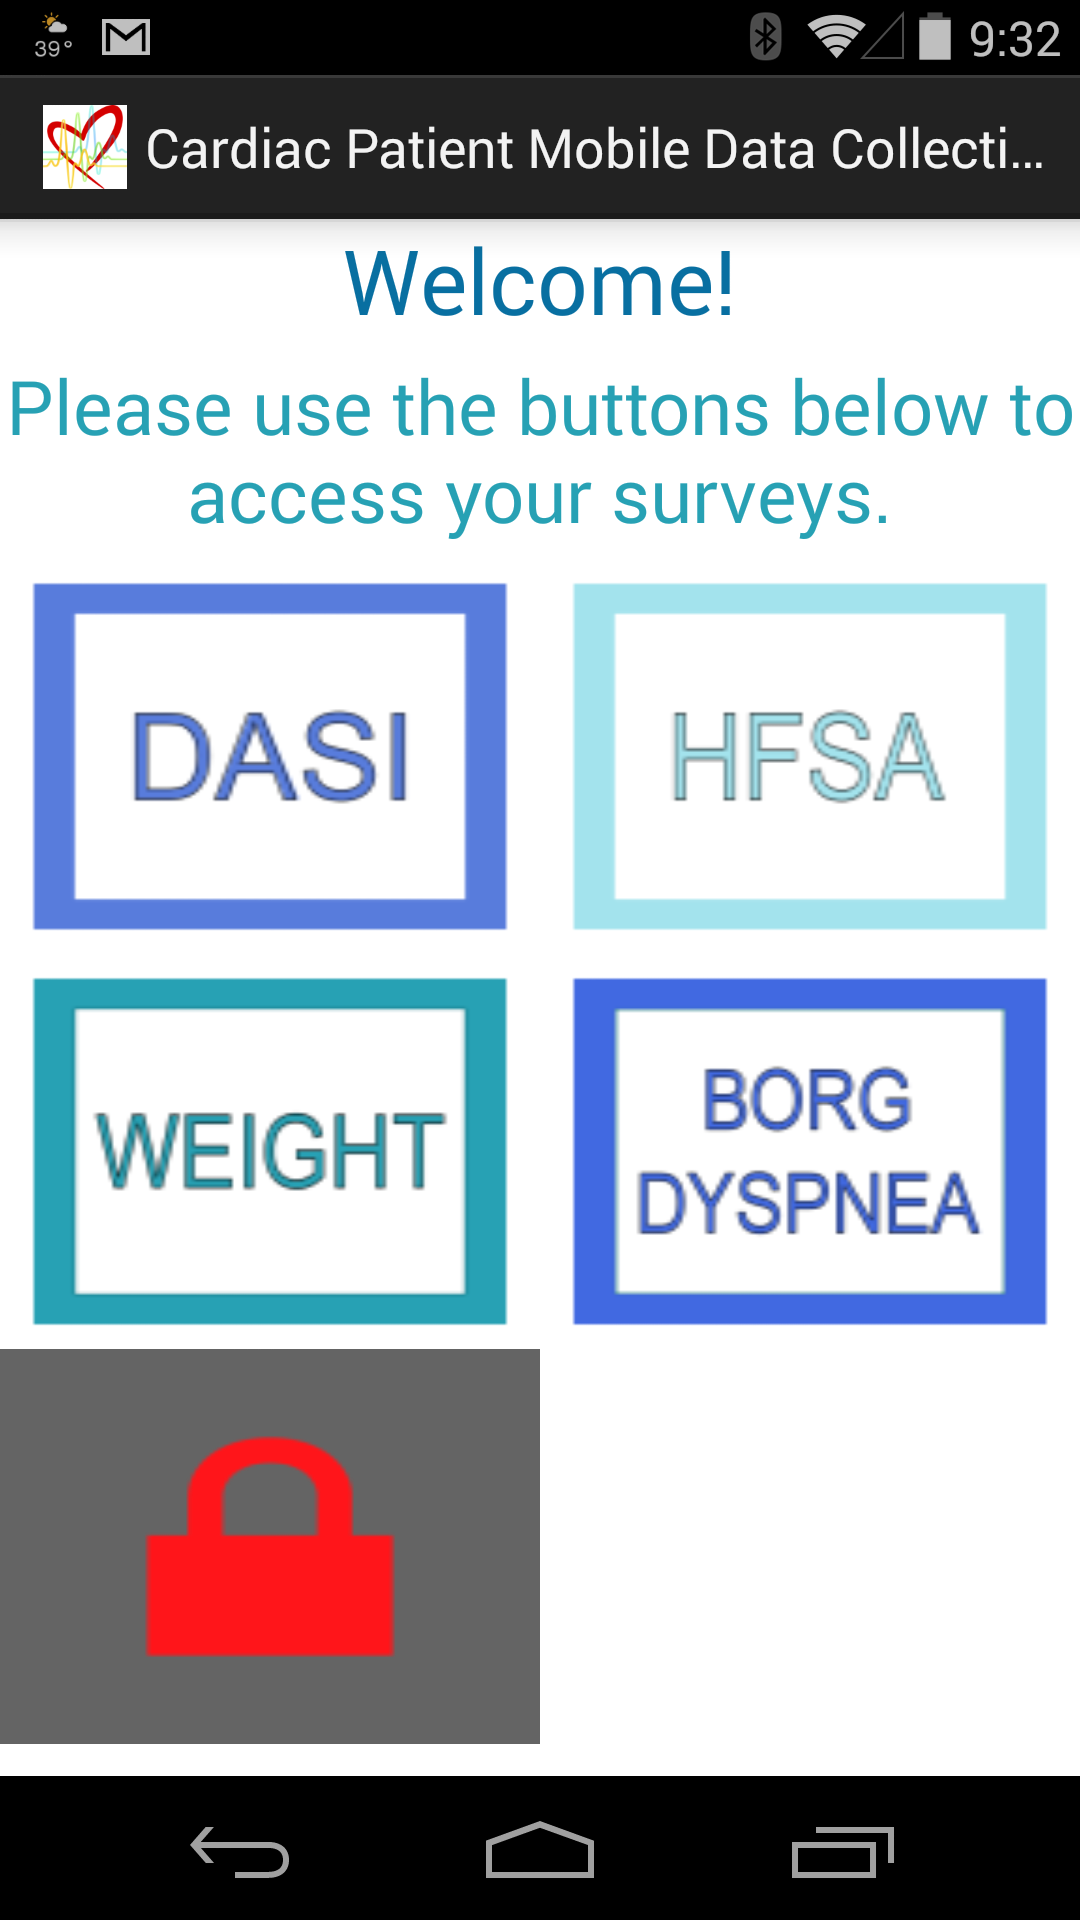
\includegraphics[scale=1,width=0.3\textwidth]{Images/AndroidSplash.png} 
  \caption{Main Screen for Smartphone Apps} 
 \end{center}
\end{figure}

\section{The Phone Application}

The smartphone application was written in Java by an undergraduate researcher, based on previous masters projects in the MCHM research group \cite{Louro2013,Putin2011}. The application underwent several revisions over the course of the trial. \cref{fig:AndroidSplash} shows the initial screen presented to enrolled patients when they started the app. allowing for weight and dispnea data entry or to trigger a psychosocial survey.

The first iteration implemented a different version of one of the psychosocial assessment tools, using a 1-4 lickert scale, the instrument was supposed to have 0-5 with 0 indicating ``I did not have that symptom''. It also did not have the self reporting behaviors for COPD patient. Last, there was no alarm feature implemented inside the survey application to remind the patients to participate in the self care instruments.

\begin{figure}[ht]
\centering
  
  \begin{subfigure}[b]{0.3\textwidth}
  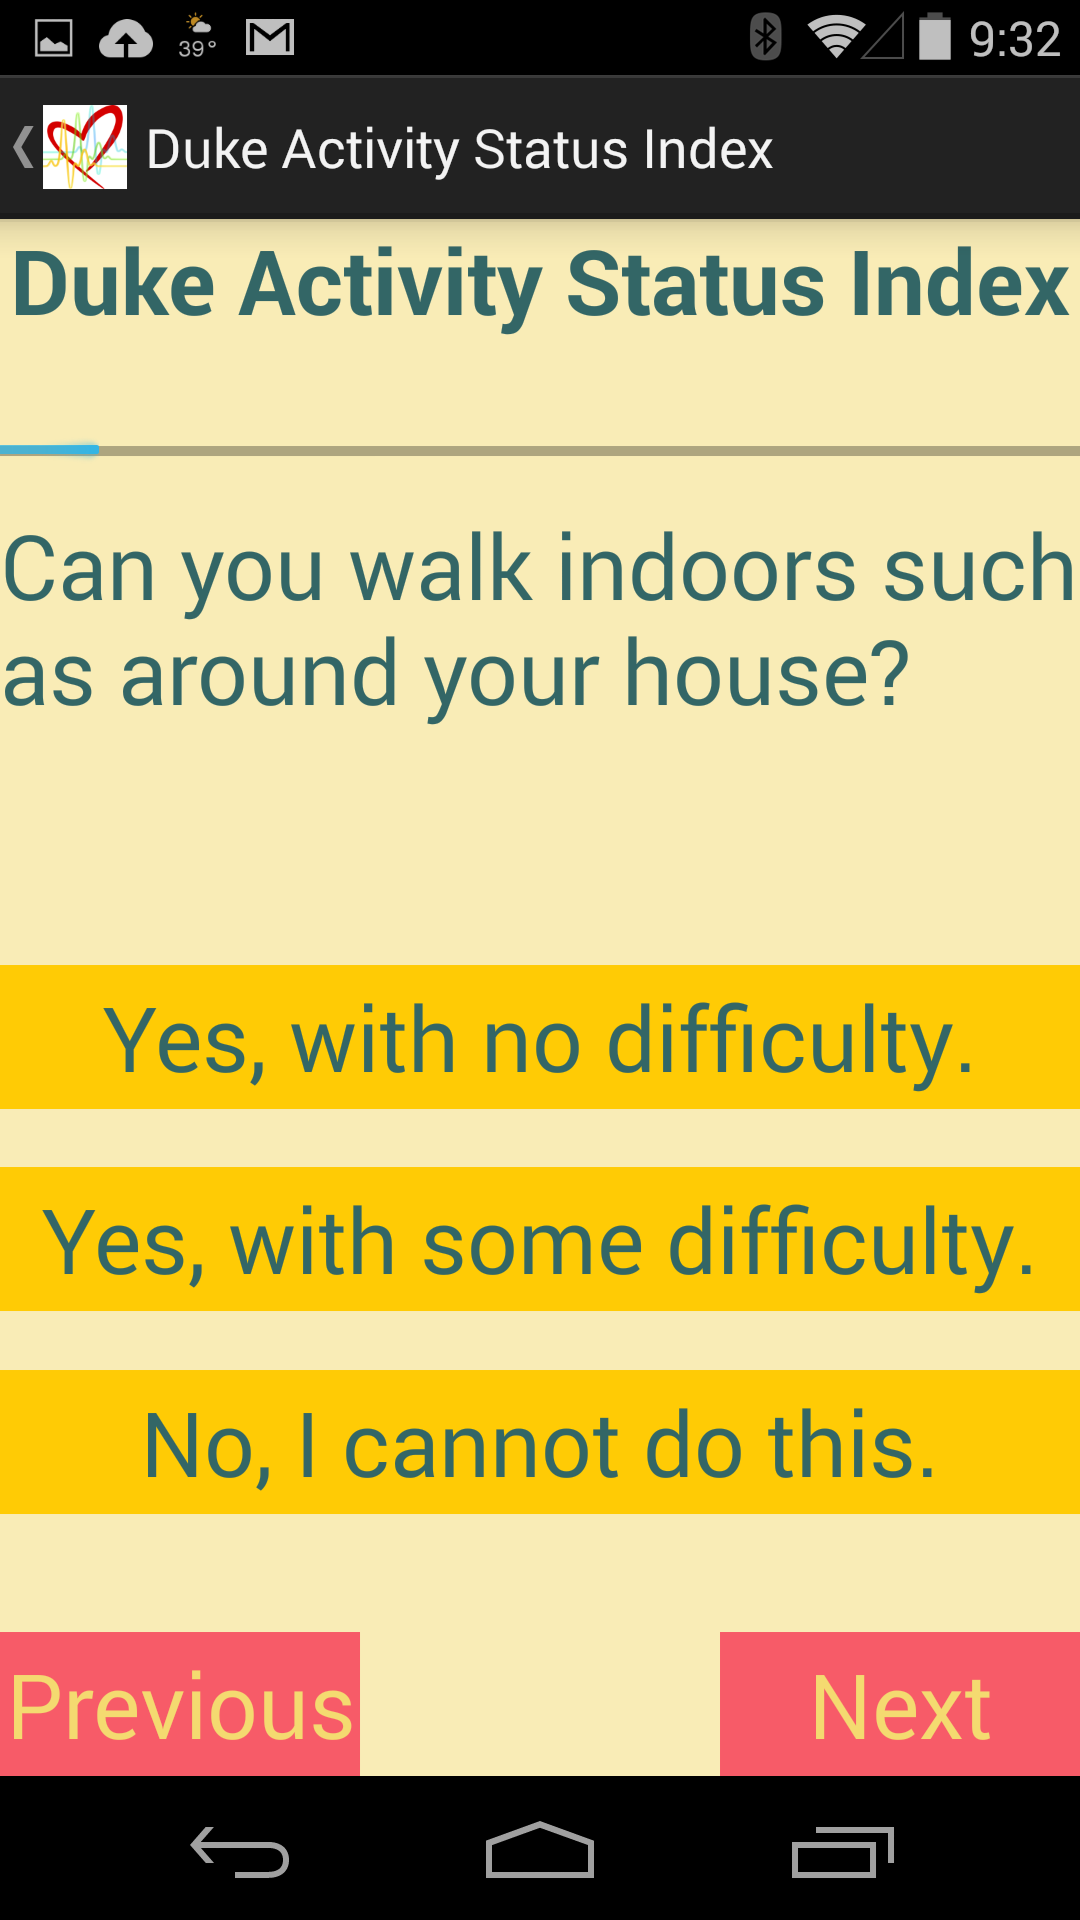
\includegraphics[scale=1,width=\textwidth]{Images/DASI.png}
  \caption{DASI Survey}
  \label{fig:DASI}
  \end{subfigure}
  ~
  \begin{subfigure}[b]{0.3\textwidth}
    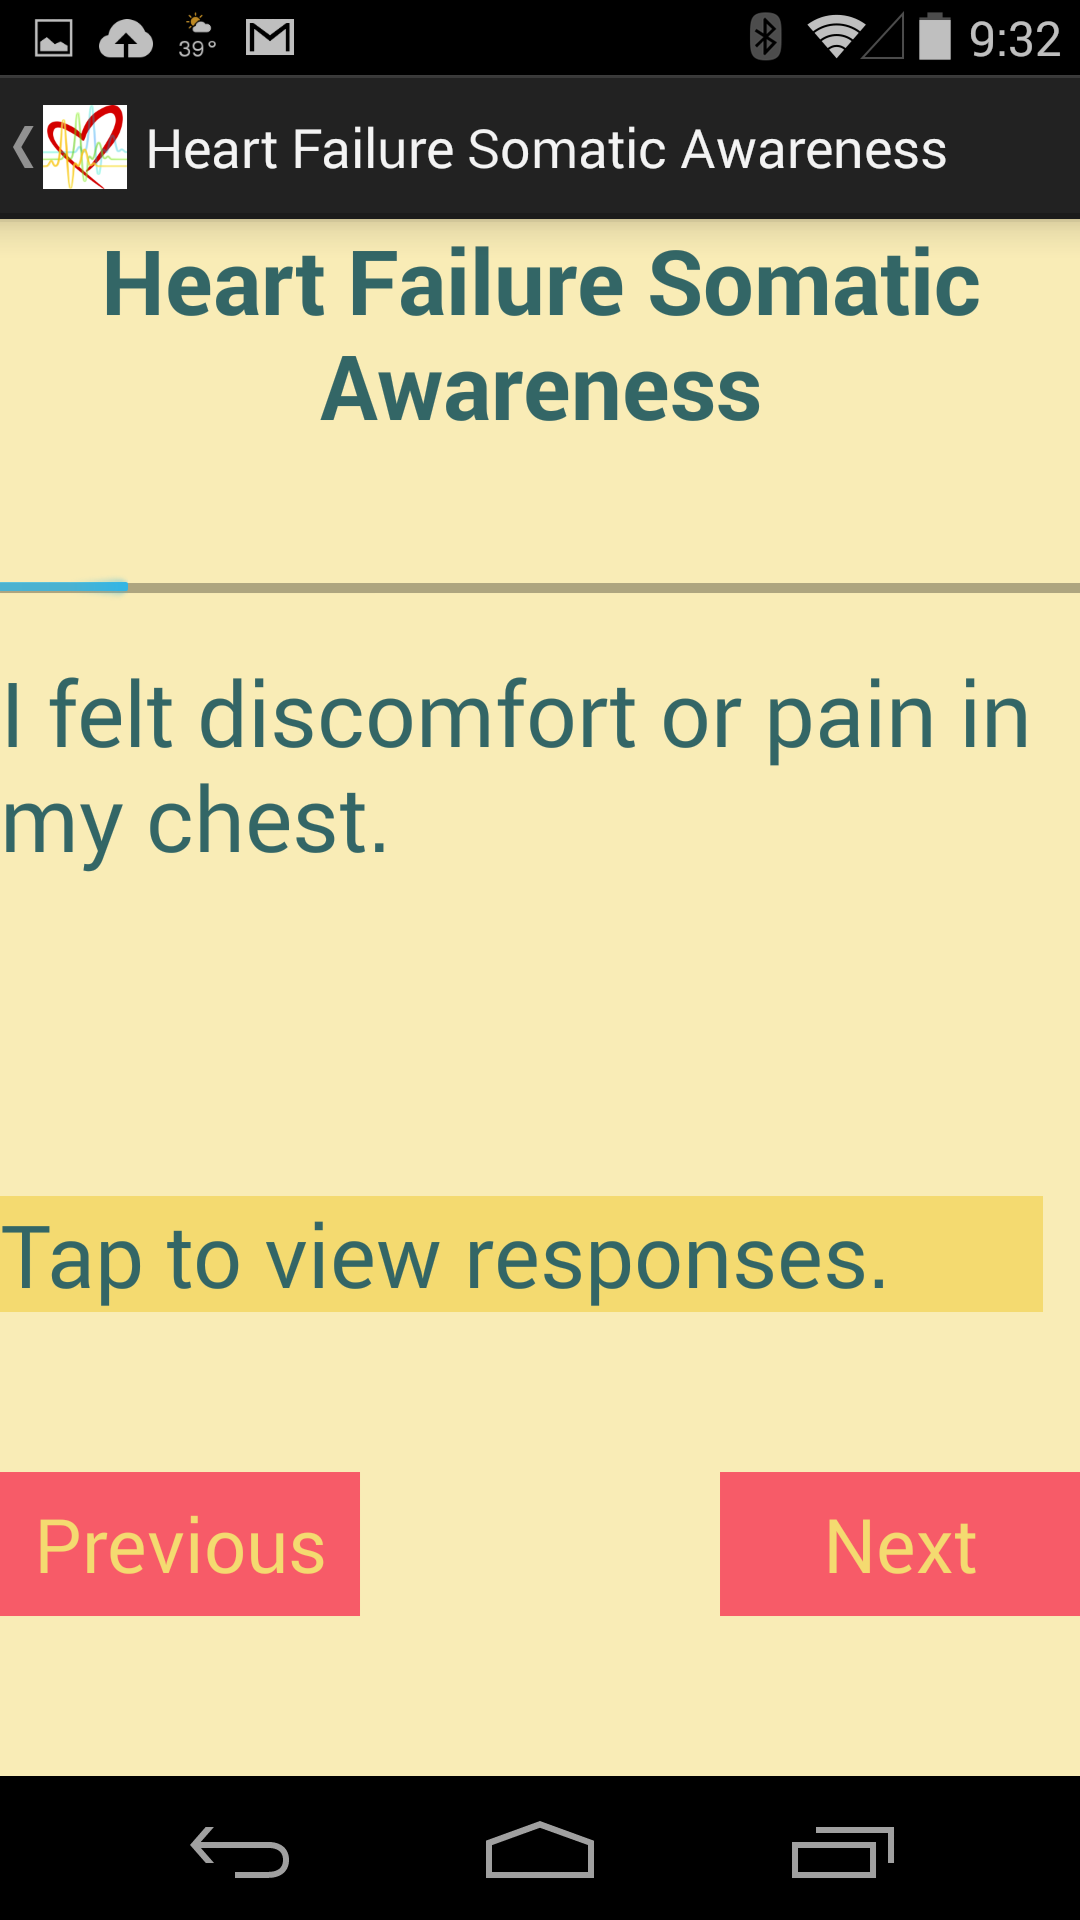
\includegraphics[scale=1,width=\textwidth]{Images/HFSA_question.png}
	\caption{HFSA Question}
  	\label{fig:HFSA_Q}
  \end{subfigure}
  ~
  \begin{subfigure}[b]{0.3\textwidth}
    	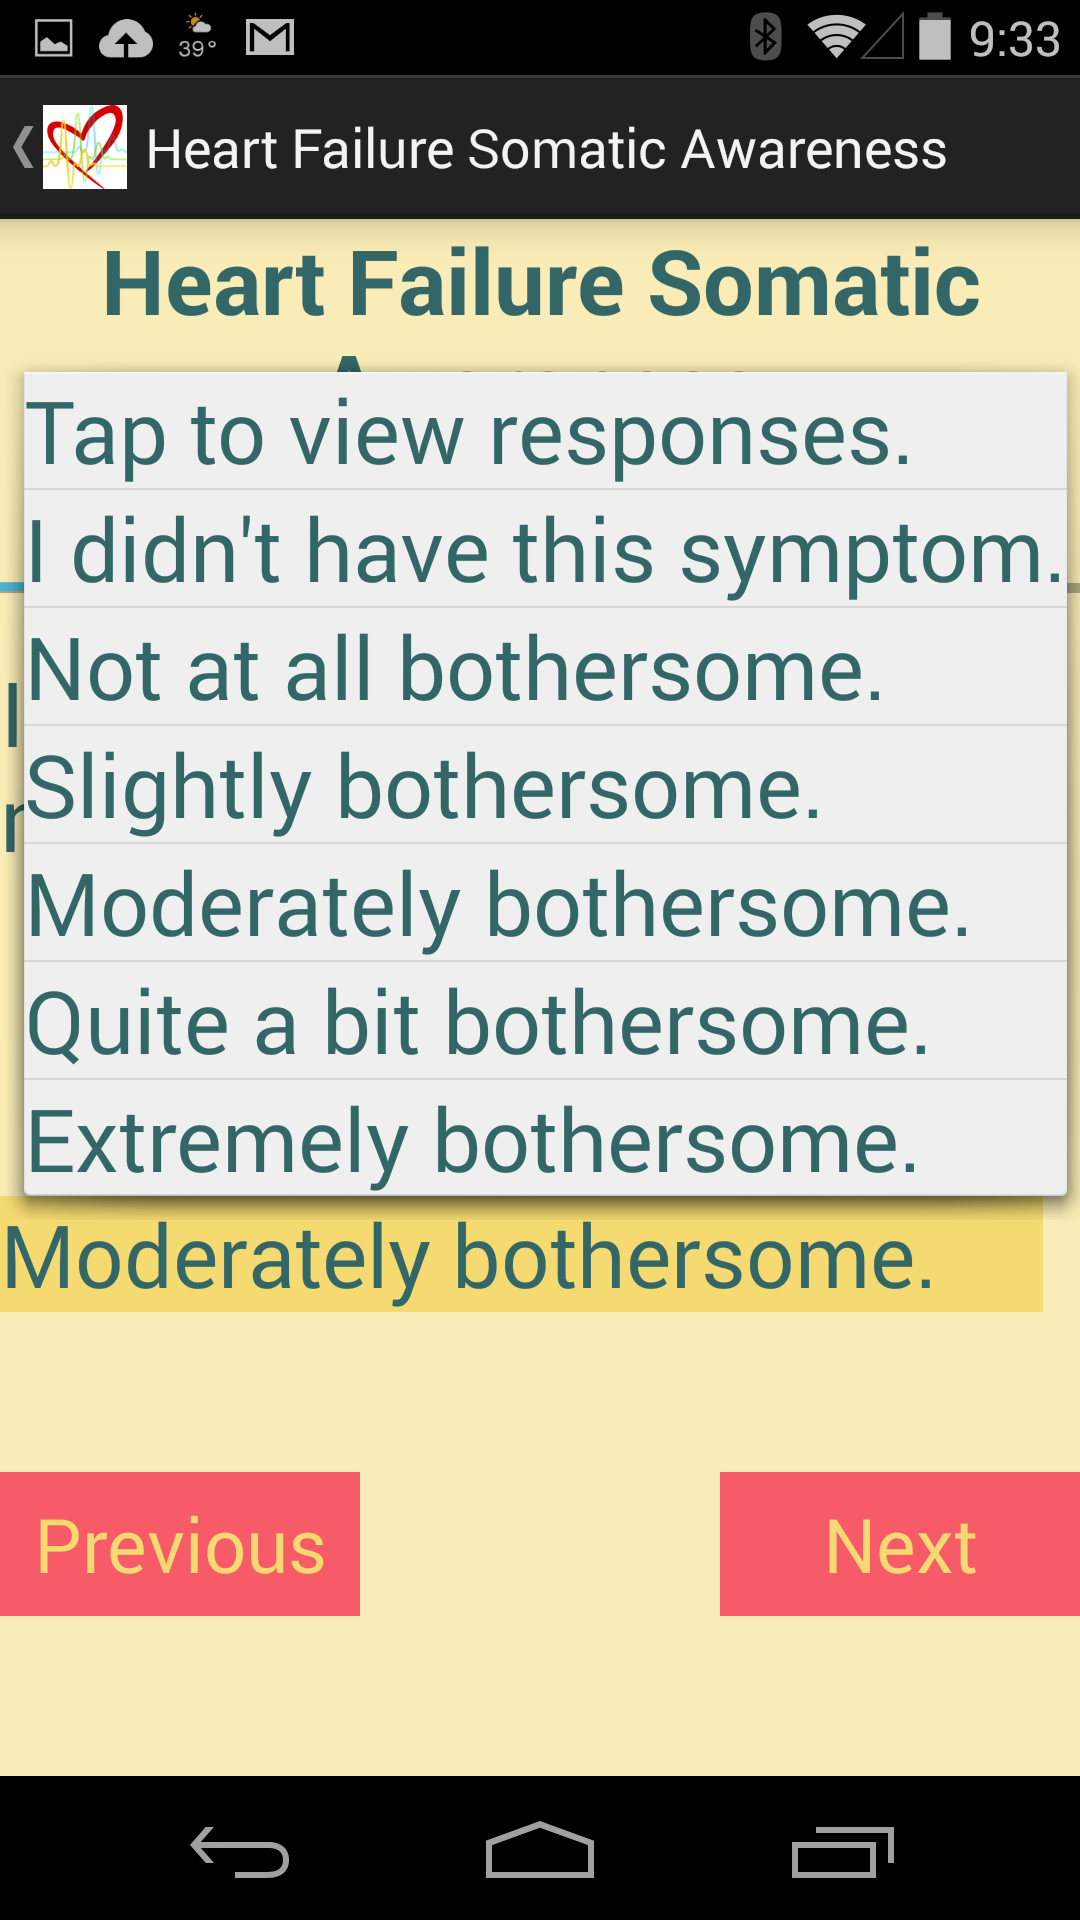
\includegraphics[scale=1,width=\textwidth]{Images/HFSA_answer.png}
  		\caption{HFSA Responses}
  		\label{fig:HFSA_R}
  \end{subfigure}
  \caption{Psychosocial Entry Screens} 
  \label{fig:AndroidSurveys}
\end{figure}

The timing of when the surveys should be administered was a reoccurring problem. Initially the phones clock alarm was used to remind the patients of when the surveys should be taken. This came to a sudden halt when one patient was unable to deactivate the alarm, only snooze it for 15 minutes at a time, for 3 days. The decision was made to remove the alarm feature from the protocol after this patient. Additionally, at the start of the trial, the patients were not allowed to take the survey instruments more than 3 times a week, as indicated by the initial proposal. However, the resulting user experience was suboptimal, the prevailing reaction to being unable to take a survey was the perception the patient had done something wrong, resulting in frustration. A modification was made to allow the surveys to be taken at any time.

Unfortunately, integrating the required fixes for the changed lickert scale introduced an error in the submission process for the HFSA instrument that went unnoticed for several months. It was ultimately fixed but the patient information was un recoverable.

Each survey was administered one question at a time, the different types of surveys each required a unique data entry technique as seen in \cref{fig:AndroidSurveys}. For the DASI, \cref{fig:DASI}, three buttons were available, pressing one, both chose the answer and advanced to the next question. For the HFSA, \cref{fig:HFSA_Q}, a dropdown box would be available to select an answer, \cref{fig:HFSA_R}, then the user would have to manually advance to the next question. 



\section{Trial Lessons Learned}

While the WHIP sensor system was the primary focus of the dissertation, the information gathered during the exploratory trial was just was important. Recording what went wrong is just as important as recording the primary data. The primary data collected was the biometric data, consisting of ECG and \spo2, and the psychosocial data, consisting of the DASI and HFSA instruments. 

\subsection{Lack of Time}
The largest obstacle present during the pre-study period, was time. Due to the urgency of the funding situation, several parts of the system were scaled back.  First, there was not time to integrate live result uploads into the WHIPPED system. Therefore, no back-end processing was performed on the real time data. Also, by not taking advantage of the wireless link between cellphone and WHIP sensor, the trial protocol was modified to include weekly visits to the patients to collect data on SD cards and replace them with empty cards. Additionally, the wireless link was supposed to allow for firmware updates of the WHIP sensor if needed. Removing the wireless link these features were deferred for the exploratory study.

In a traditional design cycle for a product, testing, or validation, may be the last step; but, it is the most important. Most designs go through several stages of testing. Alpha testing usually occurs in a lab setting where environmental factors are carefully controlled. Logical errors can usually be spotted and eliminated, in alpha testing. Beta testing widens the scope of tests, bringing the Device Under Test outside of the lab but controlling the population; limiting the population to participants who are familiar with the technology. Beta testing can be a much longer test procedure. However, to comply with the grant timing requirements. Both the device and the smart phone application were pushed into service without any beta testing. 

Another piece of the design which needed to be rushed was the wearable design. Using the polar heart strap was a decision born of expedience. It was faster to buy off the shelf straps and modify them to fit the needs of the grant. A less polished physical design was the result.

\subsection {Lost Data}
The primary goal of the WHIPPED system, after adjustments due to grant timing, was data collection. Several lessons were learned during the study. The sensor system was designed to record a theoretical maximum of eight-twelve-hour days. Originally, this was viewed as a comfortable margin of error since a nightly wireless data dump was envisioned at design time. Once the wireless link was removed from the study, a new protocol was put in place, data would be downloaded via the USB interface of the WHIP sensor. Someone would go to each participant each week with a computer and manually download the data.

The USB approach was quickly abandoned, due to speed. The USB hardware interface was only capable of full-speed USB (12 Megabits (Mb)/sec). Given that each 2 hour ECG and \spo2 datafile was approximately 100 MegaBytes (MB), one weeks worth of data would have taken $ 7 \frac{days}{week} * 8 \frac{hours}{day} * 100 \frac{MB}{2 hours} * 12 \frac{Mb}{Second} = 31.1 \frac{minutes}{week}$ to transfer data. In the future, if a microcontroller with a hi-speed USB interface is used, the same transfer would only take $ 7 \frac{days}{week} * 8 \frac{hours}{day} * 100 \frac{MB}{2 hours} * 480 \frac{Mb}{second} = 47 \frac{seconds}{week}$.  

Regardless of future implementations, the end result for the exploratory study, was that the SD cards were exchanged each week. 
Exchanging SD cards weekly led to a new set of problems. First, the one week limit on data storage was not explained to the study administrators, as a result, some patient data was lost when more than eight days elapsed between visits and the starting data was over written. This was later explained in more detail, and rectified, but the data was irretrievable. 

SD cards proved to be not able to handle the frequent handling and travel the exploratory study required. Two major sources of lost data involved the excess handling of sd cards and handling of the SD card to USB adapter used to download data from the sd card to a computer.

SD card readers require an external interface to transfer data to a computer. Several SD-to-USB converters were purchased for the purposes of the exploratory trial. At some point of during the trial one converter suffered a failure that went undiscovered for several weeks. Data files were transfered but files contained random data. When the same SD card was put into a different reader, the data was valid. To keep things as simple as possible the decision was made to no, longer use sd card adapters to download data, instead data cards would be exchanged for fresh cards and delivered for transfer where the data could be verified. This led to another problem related to the SD cards.

Like most electronic devices sd cards are sensitive to electro-static discharge (ESD). SD cards should be kept in a ESD-safe case when not inserted into a device. During the exploratory study, that was not always the case. 
As a result, entire sd cards worth of data were corrupted.

In future iterations, if wireless transfer is not available, the SD card protocol should be clearly documented. Additionally, a utility to visualize the data immediately after download would add a confidence factor for the study workers during home visits.


%\paragraph {too long between visits}
%\paragraph {bad SDcard adapter}
%\paragraph{excessive SD card handling}

\subsection{Lack of Documentation}
Lack of time had the additional effect of leaving no time for writing documentation for either the nursing faculty or the patients who would be using the device. All training was done in person. Future studies should have at least:
\begin{itemize}
\item a smartphone user manual.
\item a WHIP troubleshooting guide
\end{itemize}

A manual could take the form of written booklet, on-line video, or both. 
While the focus of the aforementioned items is on the patient and clinician, the need for manuals for engineers engaged in multidisciplinary work is even more acute. Specifically, when implementing the psychosocial instruments, great care was taken to ensure that data was validated before being inserted into the database. However, the sample space of possible answers was not made clear from the sample form provided. The one-to-five lickert scale could also contain responses such as ``does not apply'' or fractional values, such as ``0.5''. This lack of documentation resulted in many patches to the smartphone application, slowing down the trial. In the future it may be useful to have engineers that will be instrumenting similar psychosocial instruments follow on with clinician as they administer the surveys. If it is not possible to accompany clinicians, it may also be beneficial to collect a large dataset of filled in forms. Analysis of collected forms may also avoid confusion.

%\paragraph{cellphone user manual}
%\paragraph{WHIP troubleshooting guide}
%\paragraph{ digital surveys vs soft surveys}

%\subsection{Communication Problems}

%\subsubsection{patient - nurse communication}
%\paragraph{cellphone usage}
%\paragraph{proper strap placement/usage}

%\subsubsection{Feature creep}
%\paragraph{COPD - Borg Dispnea}
%\paragraph{modified likert}
%\paragraph{survey alarms}
%\paragraph{strict survey -> anytime survey}

%\subsubsection{nurse - engineer communication}
%\paragraph{delay between problem observation and problem reporting}
%\paragraph{no timely feedback on collected data}


%\subsection{Loose protocol adherence}
%\paragraph{ changes in survey protocol, database changes}
%\paragraph{ changes in sensor useage (finger clip)}
%\paragraph{ no calibration measurements}
%\paragraph{ ECG Disconnected}
